\documentclass[aspectratio=169,9pt]{beamer}

\usepackage{graphicx,caption,subcaption,hyperref,amsmath,amsfonts,amssymb,appendixnumberbeamer,makecell,tikz,tikz-cd}
\usetikzlibrary{matrix,arrows,positioning,calc,shapes,arrows.meta,automata,cd}
\usepackage[normalem]{ulem}
\graphicspath{ {./figures/} }
% \captionsetup{font=scriptsize,labelfont=scriptsize}
\setbeamerfont{footnote}{size=\scriptsize}
\usepackage[strict]{changepage}
\usetheme[titleformat=smallcaps,
            sectionpage=progressbar,
			subsectionpage=progressbar,
			progressbar=frametitle,
			numbering=fraction]{metropolis}

% \usecolortheme{owl}
\usepackage[style=apa,
			sorting=nyt,
			date=year,
			bibencoding=utf8,
			isbn=false,
			eprint=false,
            doi=false,
			dashed=false,
			uniquelist=false,
			maxbibnames=2,
			minbibnames=1,
			maxcitenames=2,
			uniquename=init,            
			giveninits=true,
			useprefix=false,
			minsortnames=1,
			maxsortnames=2]{biblatex}
\usepackage{appendixnumberbeamer}
\DeclareCiteCommand{\cite}
  {\printfield{prenote}}
  {\printnames{labelname}
  \ifentrytype{article}
    {\newunit{\addcomma}\printfield{journaltitle}}
    {}%
  \newunit{\addcomma}
  \printfield{labelyear}%
  }
  {\addsemicolon\addspace}
  {\printfield{postnote}}
  
\bibliography{MBF}
\renewcommand{\thefigure}{\hspace{-.25em}}
\renewcommand{\thetable}{\hspace{-.25em}}

\setsansfont[BoldFont={Fira Sans SemiBold}]{Fira Sans Book}

\newcommand{\bbB}{\mathbb{B}}
\newcommand{\cL}{\mathcal{L}}
\newcommand{\bL}{\mathbb{L}}
\newcommand{\bU}{\mathbb{U}}
\newcommand{\boolf}{{\mathfrak 0}}
\newcommand{\boolt}{{\mathfrak 1}}
\newcommand{\Targets}{\mathbf{T}}
\newcommand{\Sources}{\mathbf{S}}
\newcommand{\bzero}{{\bf 0}}
\newcommand{\bone}{{\bf 1}}

% \newtheorem{theorem}{Theorem}

\theoremstyle{definition}
\newtheorem{defn}{Definition}
\theoremstyle{remark}
\newtheorem*{remark}{Remark}

\newcounter{countitems}

\newcommand{\red}[1]{{
\color{red}
{#1}}} 

\title{Fixed points and multistability in monotone Boolean network models}
\author{Harshavardhan BV}
\institute{IMI, IISc Bengaluru}
\date{\today}

\begin{document}

\maketitle

\begin{frame}{In collaboration with}
\begin{figure}
    \centering
    \begin{subfigure}{0.4\textwidth}
        \centering
        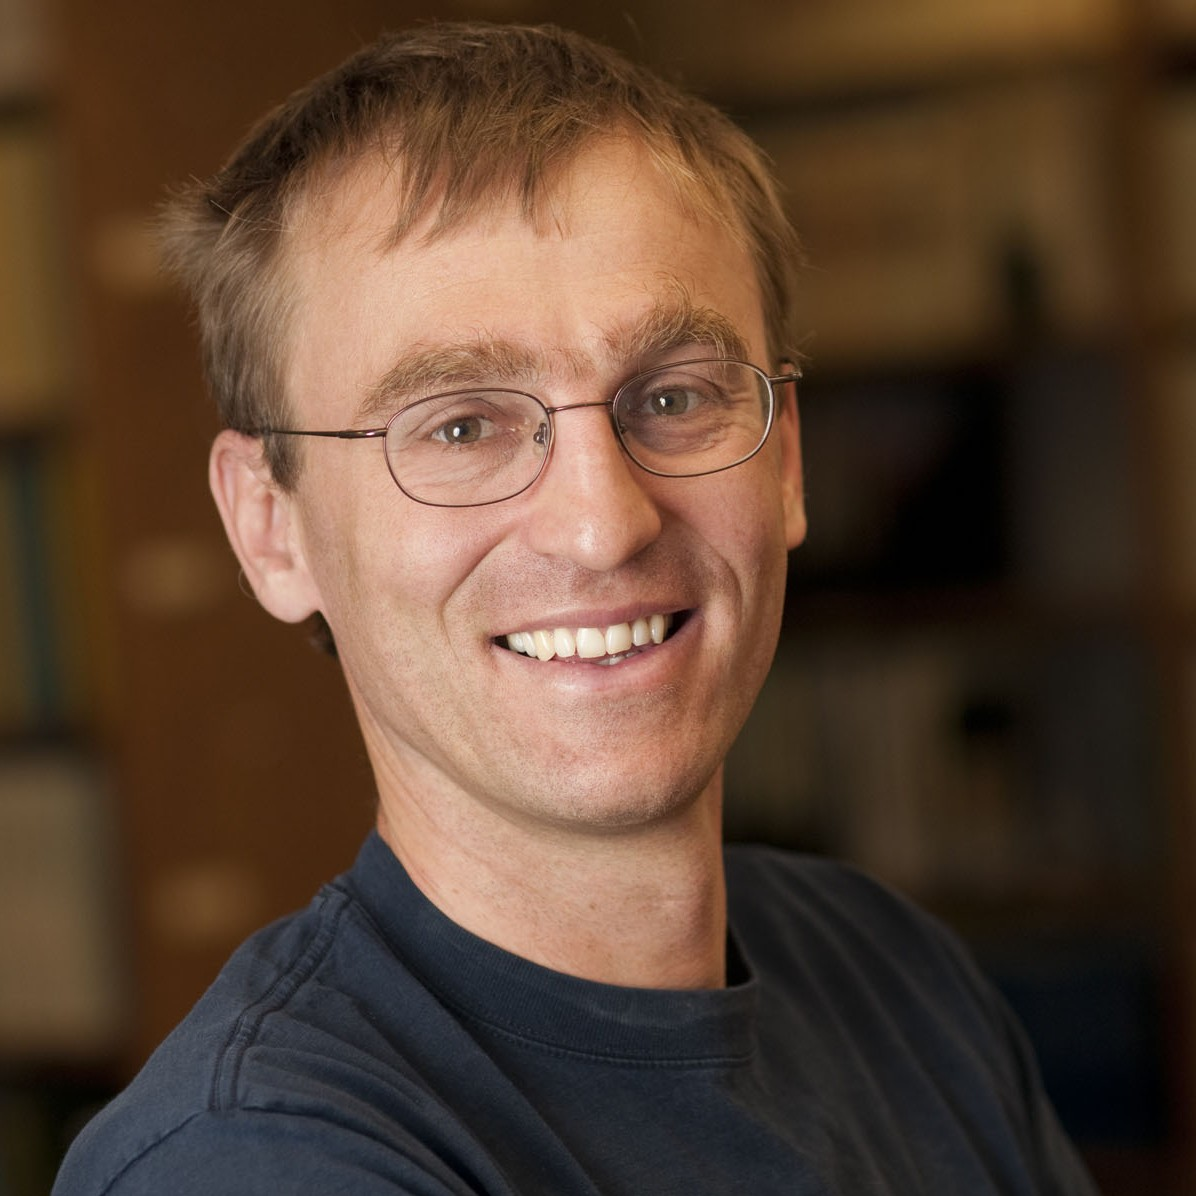
\includegraphics[width=\textwidth]{figures/Tomas.jpg}
        \caption*{Tomas Gedeon, Montana State University}
    \end{subfigure}
    \begin{subfigure}{0.4\textwidth}
        \centering
        
\includegraphics[width=\textwidth]{figures/Sarah.jpg}
        \caption*{Sarah Adigwe, Montana State University}
    \end{subfigure}
\end{figure}
\end{frame}

% \section{Introduction}

\begin{frame}{Modeling Gene Regulation}
\begin{adjustwidth}{-5cm}{-5cm}
\begin{columns}
    \begin{column}{0.4\textwidth}
        \begin{figure}
            \centering
            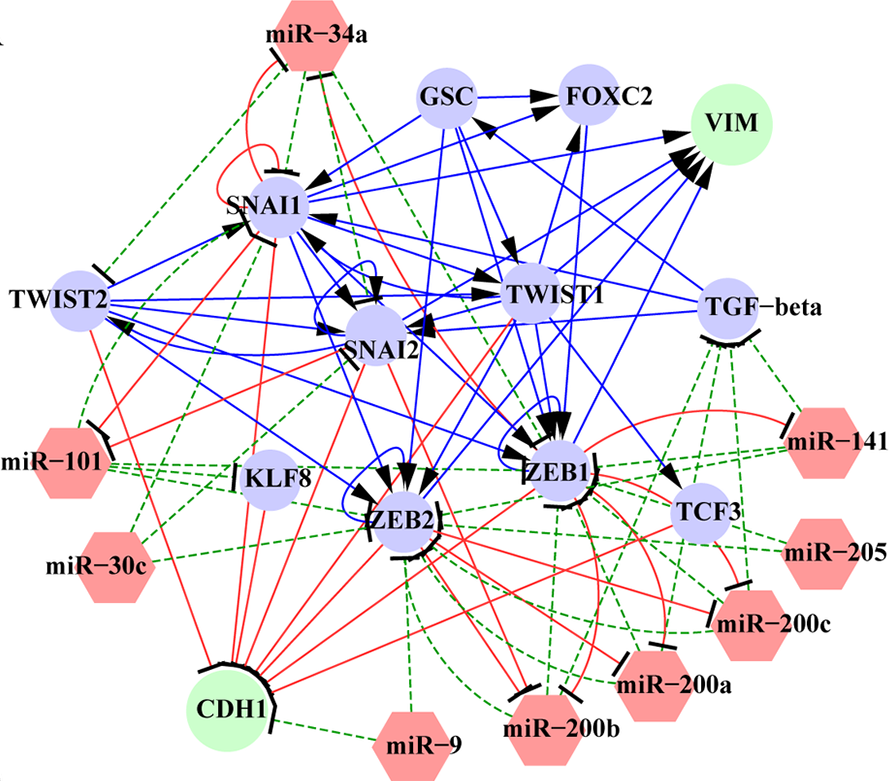
\includegraphics[width=\linewidth]{figures/EMT.png}
            \caption{EMT network\footnotemark[1]}
        \end{figure}
    \end{column}
    \begin{column}{0.6\textwidth}
    \only<2>{
        ODE:
        \begin{align*}
        \frac{dX_1}{dt} &= g_1 H^{s+}(\cdot)H^{s-}(\cdot) - k_1 X_1 \\
        &\vdots \\
        \frac{dX_N}{dt} &= g_N H^{s+}(\cdot)H^{s-}(\cdot) - k_N X_N
        \end{align*}
        }
    \only<3>{
        \begin{figure}
            \centering
            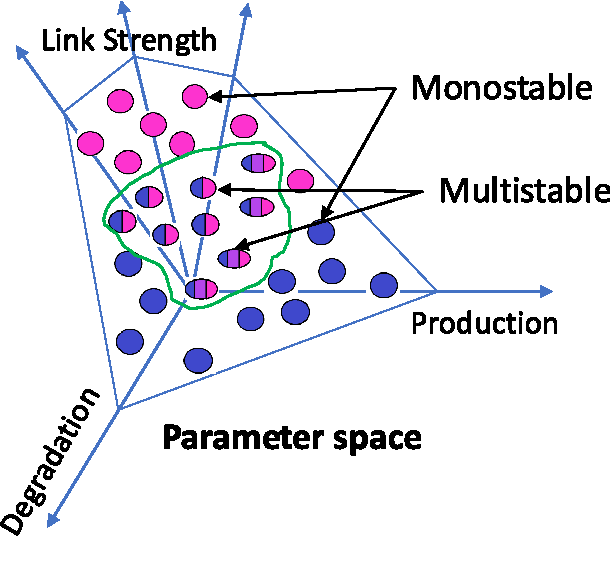
\includegraphics[width=0.7\linewidth]{figures/RACIPE_schematic.pdf}
            \caption{RACIPE: Parameter sampling\footnotemark[2]}
        \end{figure}
    }
    \only<4>{
        Boolean\footnotemark[3]:
        \begin{align*}
        X_1(t+1) &= X_1(t) \vee X_2(t) \cdots \wedge X_n(t)\\
        &\vdots \\
        X_N(t+1) &= \neg X_2(t) \dots \vee \neg X_{n-1}(t)\
        \end{align*}
    }
    \end{column}
\end{columns}
\end{adjustwidth}
\footnotetext[1]{\cite{huang_interrogating_2017,}}
\footnotetext[2]{\cite{huang_racipe_2018}. Figure by Kishore Hari}
\footnotetext[3]{\cite{albert_boolean_2014}}
\end{frame}

\begin{frame}{Monotone Boolean Functions (MBFs) and Models (MBMs)}
\begin{defn}
A Boolean function $f \colon \bbB^k \to \bbB$ is \emph{increasing with respect to input $j$} if for any input $b=(b_1, \ldots, b_k) \in \bbB^k$
\[
f(b_1, \ldots, b_{j-1}, 0, b_{j+1}, \ldots, b_k) \leq f(b_1 \ldots, b_{j-1}, 1, b_{j+1}, \ldots, b_k).
\]
\end{defn}

\begin{defn}
A Boolean function $f \colon \bbB^k \to \bbB$ is \emph{monotone} if it is increasing or decreasing with respect to each input $i=1, \ldots, k$. In this case, $f$ is called a \emph{monotone Boolean function}.

A set of increasing monotone Boolean functions $f \colon \bbB^k \to \bbB$ will be denoted $MBF(k)$. 
\end{defn}

\begin{defn}
A Boolean model $f \colon \bbB^N \to \bbB^N, f=(f_1, \ldots, f_N)$, is \emph{monotone} if for every $i$ the function $f_i$ is monotone.
\end{defn}

\footnotetext[1]{\cite{gedeon_network_2024, korshunov_monotone_2003}}
\end{frame}

\begin{frame}{MBF(1)}
\begin{adjustwidth}{-5cm}{-5cm}
    \only<1-3>{
    \begin{figure}
        \centering
        \begin{subfigure}[c]{0.25\textwidth}
            \centering
            \begin{tikzpicture}[main node/.style={circle,fill=white!20,thick,draw},scale=1.5]
                \node[main node] (1) at (0,0) {A};
                \node[main node] (2) at (1,0) {B};
                \node[main node, fill=yellow] (3) at (0,-1) {A};
                \node[main node] (4) at (1,-1) {B};
                \path[thick] (1) edge[->, color=red,shorten <= 2pt, shorten >= 2pt] (2);
                \path[thick] (3) edge[->, color=red,shorten <= 2pt, shorten >= 2pt] (4);
            \end{tikzpicture}
        \end{subfigure}
        \begin{subfigure}[c]{0.25\textwidth}
            \centering
            \begin{tikzpicture}[main node/.style={circle,fill=white!20,thick,draw},scale=1.5]
                \node[main node] (1) at (0,0) {A};
                \node[main node, fill=yellow] (2) at (1,0) {B};
                \node[main node, fill=yellow] (3) at (0,-1) {A};
                \node[main node, fill=yellow] (4) at (1,-1) {B};
                \path[thick] (1) edge[->, color=red,shorten <= 2pt, shorten >= 2pt] (2);
                \path[thick] (3) edge[->, color=red,shorten <= 2pt, shorten >= 2pt] (4);
            \end{tikzpicture}
        \end{subfigure}
        \pause
        \begin{subfigure}[c]{0.25\textwidth}
            \centering
            \begin{tikzpicture}[main node/.style={circle,fill=white!20,thick,draw},scale=1.5]
                \node[main node] (1) at (0,0) {A};
                \node[main node] (2) at (1,0) {B};
                \node[main node,fill=yellow] (3) at (0,-1) {A};
                \node[main node,fill=yellow] (4) at (1,-1) {B};
                \path[thick] (1) edge[->, color=red,shorten <= 2pt, shorten >= 2pt] (2);
                \path[thick] (3) edge[->, color=red,shorten <= 2pt, shorten >= 2pt] (4);
            \end{tikzpicture}
        \end{subfigure}
        \pause
        \begin{subfigure}[c]{0.2\textwidth}
            \centering
            \begin{tikzpicture}[main node/.style={circle,fill=white!20,thick,draw},scale=1.5]
                \node[main node] (1) at (0,0) {A};
                \node[main node,fill=yellow] (2) at (1,0) {B};
                \node[main node,fill=yellow] (3) at (0,-1) {A};
                \node[main node] (4) at (1,-1) {B};
                \path[thick] (1) edge[->, color=red,shorten <= 2pt, shorten >= 2pt] (2);
                \path[thick] (3) edge[->, color=red,shorten <= 2pt, shorten >= 2pt] (4);
                \draw[red, ultra thick] (-0.3,0.3) -- (1.3,-1.3);
                \draw[red, ultra thick] (-0.3,-1.3) -- (1.3,0.3);
            \end{tikzpicture}
        \end{subfigure}
        \pause[1]\caption{Schematic of increasing MBF(1) for activatory input}
    \end{figure}}
    \only<4>{
    \begin{figure}
        \centering
        \begin{subfigure}[c]{0.25\textwidth}
            \centering
            \begin{tikzpicture}[main node/.style={circle,fill=white!20,thick,draw},scale=1.5]
                \node[main node] (1) at (0,0) {A};
                \node[main node] (2) at (1,0) {B};
                \node[main node, fill=yellow] (3) at (0,-1) {A};
                \node[main node] (4) at (1,-1) {B};
                \path[thick] (1) edge[-|, color=blue,shorten <= 2pt, shorten >= 2pt] (2);
                \path[thick] (3) edge[-|, color=blue,shorten <= 2pt, shorten >= 2pt] (4);
            \end{tikzpicture}
        \end{subfigure}
        \begin{subfigure}[c]{0.25\textwidth}
            \centering
            \begin{tikzpicture}[main node/.style={circle,fill=white!20,thick,draw},scale=1.5]
                \node[main node] (1) at (0,0) {A};
                \node[main node, fill=yellow] (2) at (1,0) {B};
                \node[main node, fill=yellow] (3) at (0,-1) {A};
                \node[main node, fill=yellow] (4) at (1,-1) {B};
                \path[thick] (1) edge[-|, color=blue,shorten <= 2pt, shorten >= 2pt] (2);
                \path[thick] (3) edge[-|, color=blue,shorten <= 2pt, shorten >= 2pt] (4);
            \end{tikzpicture}
        \end{subfigure}
        \begin{subfigure}[c]{0.25\textwidth}
            \centering
            \begin{tikzpicture}[main node/.style={circle,fill=white!20,thick,draw},scale=1.5]
                \node[main node] (1) at (0,0) {A};
                \node[main node, fill=yellow] (2) at (1,0) {B};
                \node[main node, fill=yellow] (3) at (0,-1) {A};
                \node[main node] (4) at (1,-1) {B};
                \path[thick] (1) edge[-|, color=blue,shorten <= 2pt, shorten >= 2pt] (2);
                \path[thick] (3) edge[-|, color=blue,shorten <= 2pt, shorten >= 2pt] (4);
            \end{tikzpicture}
        \end{subfigure}
        \begin{subfigure}[c]{0.25\textwidth}
            \centering
            \begin{tikzpicture}[main node/.style={circle,fill=white!20,thick,draw},scale=1.5]
                \node[main node] (1) at (0,0) {A};
                \node[main node] (2) at (1,0) {B};
                \node[main node,fill=yellow] (3) at (0,-1) {A};
                \node[main node,fill=yellow] (4) at (1,-1) {B};
                \path[thick] (1) edge[-|, color=blue,shorten <= 2pt, shorten >= 2pt] (2);
                \path[thick] (3) edge[-|, color=blue,shorten <= 2pt, shorten >= 2pt] (4);
                \draw[red, ultra thick] (-0.3,0.3) -- (1.3,-1.3);
                \draw[red, ultra thick] (-0.3,-1.3) -- (1.3,0.3);
            \end{tikzpicture}
        \end{subfigure}
        \caption{Schematic of decreasing MBF(1) for inhibitory input}
    \end{figure}}
\end{adjustwidth}
\end{frame}

\begin{frame}[noframenumbering]{MBF(2)}
\only<1-2>{
\begin{table}[h!]
\centering
\only<1>{
\begin{tabular}{|c|c|c|c|c|c|c|c|c|c|c|c|c|c|c|c|c|c|}
\hline
\multicolumn{2}{|c|}{\textbf{Inputs}} & \multicolumn{16}{|c|}{\textbf{BFs}}\\ \hline
$X$ & $Y$ & \multicolumn{16}{|c|}{}\\ \hline
0 & 0 & 0 & 0 & 0 & 0 & 0 & 0 & 0 & 0 & 1 & 1 & 1 & 1 & 1 & 1 & 1 & 1 \\
0 & 1 & 0 & 0 & 0 & 0 & 1 & 1 & 1 & 1 & 0 & 0 & 0 & 0 & 1 & 1 & 1 & 1 \\
1 & 0 & 0 & 0 & 1 & 1 & 0 & 0 & 1 & 1 & 0 & 0 & 1 & 1 & 0 & 0 & 1 & 1 \\
1 & 1 & 0 & 1 & 0 & 1 & 0 & 1 & 0 & 1 & 0 & 1 & 0 & 1 & 0 & 1 & 0 & 1 \\ \hline
\end{tabular}}
\only<2>{
\begin{tabular}{|c|c|c|c|c|c|c|c|c|c|c|c|c|c|c|c|c|c|}
\hline
\multicolumn{2}{|c|}{\textbf{Inputs}} & \multicolumn{16}{|c|}{\textbf{BFs}}\\ \hline
$X$ & $Y$ & \multicolumn{16}{|c|}{}\\ \hline
0 & 0 & 0 & 0 & \red{0} & 0 & \red{0} & 0 & \red{0} & 0 & \red{1} & \red{1} & \red{1} & \red{1} & \red{1} & \red{1} & \red{1} & 1 \\
0 & 1 & 0 & 0 & \red{0} & 0 & \red{1} & 1 & \red{1} & 1 & \red{0} & \red{0} & \red{0} & \red{0} & \red{1} & \red{1} & \red{1} & 1 \\
\textbf{1} & \textbf{0} & 0 & 0 & \textbf{\red{1}} & 1 & \red{0} & 0 & \red{1} & 1 & \red{0} & \red{0} & \red{1} & \red{1} & \red{0} & \red{0} & \red{1} & 1 \\
\textbf{1} & \textbf{1} & 0 & 1 & \textbf{\red{0}} & 1 & \red{0} & 1 & \red{0} & 1 & \red{0} & \red{1} & \red{0} & \red{1} & \red{0} & \red{1} & \red{0} & 1 \\ \hline
\end{tabular}}
\caption{Table of BFs for a node with two inputs $X$ and $Y$.}
\end{table}}
\only<2>{\footnotetext[1]{Red indicates non-increasing functions (non-monotonous)}}
\only<3>{
\begin{figure}[t]
    \centering
    \begin{subfigure}[c]{0.5\textwidth}
        \centering
        \begin{tabular}{|c|c|c|c|c|c|c|c|}
        \hline
        \multicolumn{2}{|c|}{\textbf{Inputs}} & \multicolumn{6}{|c|}{\textbf{MBFs}} \\ \hline
        $X$ & $Y$ & $\bzero$ & $\vee$ & ${\bf X}$ & ${\bf Y}$ & $\wedge$ & $\bone$ \\ \hline
        0 & 0 & 0 & 0 & 0 & 0 & 0 & 1 \\
        0 & 1 & 0 & 0 & 0 & 1 & 1 & 1 \\
        1 & 0 & 0 & 0 & 1 & 0 & 1 & 1 \\
        1 & 1 & 0 & 1 & 1 & 1 & 1 & 1 \\ \hline
        \end{tabular}
    \end{subfigure}
    \begin{subfigure}{0.3\textwidth}
        \begin{tikzpicture}[node distance = .5cm,baseline=(current bounding box.center)]
            \tikzset{my node/.style = {circle, draw, thick, inner sep=4pt, minimum size=0pt}}
            \tikzset{my edge/.style = {-, very thick}}
            \node[my node] (1) { $\bone$ };
            \node[my node] (2) [below=of 1] {$\vee$};
            \node[my node] (3) [below left=0.4 and 0.2 of 2] {$X$};
            \node[my node] (4) [below right=0.4 and 0.2 of 2] {$Y$};
            \node[my node] (5) [below left=0.4 and 0.2 of 4] {$\wedge$};
            \node[my node] (6) [below=of 5] {$\bzero$};
            \draw[my edge] (1) -- (2);
            \draw[my edge] (2) -- (3);
            \draw[my edge] (2) -- (4);
            \draw[my edge] (3) -- (5);
            \draw[my edge] (4) -- (5);
            \draw[my edge] (5) -- (6);
        \end{tikzpicture}
    \end{subfigure}
\caption{Table (left) and Lattice (right) of MBF(2) for a node with two activatory inputs $X$ and $Y$.}
\end{figure}
}
\end{frame}

\begin{frame}[fragile]{Negative loop (NL)-free networks}
     \[
        \begin{tikzcd}
            \bbB^N \arrow[r, "f"] \arrow[d,"\alpha",shift left]
            & \bbB^N \arrow[d,"\alpha", shift left]\\
            \bbB^N \arrow[r, "g" ] \arrow[u,"\alpha", shift left]
            & \bbB^N \arrow[u,"\alpha", shift left] 
        \end{tikzcd}
    \]
    \pause 
    \vspace{0.25cm}
    
    Trajectories and Steady states preserved
    \[ x=f(x) \quad \Longleftrightarrow \quad \alpha(x) = g(\alpha(x)).\]
    \pause[1]
    \begin{itemize}
        \item $f=(f_1, \ldots, f_N)$: NL-free network MBM
        \item $\alpha$: Change of variable transformation 
        \item $g=(g_1, \ldots, g_N)$: Positive network MBM
    \end{itemize}
\end{frame}

\begin{frame}{Change of variable - Toggle switch}
    \begin{figure}
    \centering
    \onslide<1->{%
    \begin{subfigure}[c]{0.4\textwidth}
        \centering
        \begin{tikzpicture}[every node/.style={circle,fill=white!20,thick,draw},scale=2.5,
        blueedge/.style={thick,blue,-|,shorten <=2pt,shorten >=2pt},
        rededge/.style={thick,red,->,shorten <=2pt,shorten >=2pt},
        textbox/.style={draw=none, fill=none, midway}
        ]
            \node (A) at (0.5,1) {A};
            \node (B) at (0.5,0) {B};
            \path[blueedge, bend left] 
                (A) edge (B)
                (B) edge (A);
            \pause
            \node[fill=cyan] (AP) at (1.5,1) {A};
            \node (BP) at (1.5,0) {B};
            \path[rededge, bend left] 
                (AP) edge (BP)
                (BP) edge (AP);
            \draw[dashed, thick, ->] (0.8,0.5) -- (1.2,0.5) 
                node[textbox, above=1.2mm] {($\neg$A,B)}
                node[textbox, below=1mm] {$\alpha$};
        \end{tikzpicture}
    \end{subfigure}
    } 
    \onslide<3->{
    \begin{subfigure}[c]{0.4\textwidth}
        \centering
        \begin{tikzpicture}[every node/.style={circle,fill=white!20,thick,draw},scale=2.5,
        blueedge/.style={thick,blue,-|,shorten <=2pt,shorten >=2pt},
        rededge/.style={thick,red,->,shorten <=2pt,shorten >=2pt},
        textbox/.style={draw=none, fill=none, midway}
        ]
            \node (ASA) at (0.5,1) {A};
            \node (BSA) at (0.5,0) {B};
            \path[blueedge, bend left]
                (ASA) edge (BSA)
                (BSA) edge (ASA);
            \path[rededge, loop above, min distance=6pt]
                (ASA) edge (ASA);
            \path[rededge, loop below, min distance=6pt]
                (BSA) edge (BSA);
            \node[fill=cyan] (APSA) at (1.5,1) {A};
            \node (BPSA) at (1.5,0) {B};
            \path[rededge, bend left] 
                (APSA) edge (BPSA)
                (BPSA) edge (APSA);
            \path[rededge, loop above, min distance=6pt]
                (APSA) edge (APSA);
            \path[rededge, loop below, min distance=6pt]
                (BPSA) edge (BPSA);
            \draw[dashed, thick, ->] (0.8,0.5) -- (1.2,0.5) 
                node[textbox, above=1.2mm] {($\neg$A,B)}
                node[textbox, below=1mm] {$\alpha$};
        \end{tikzpicture}
    \end{subfigure}
    }
    \end{figure}
    \footnotetext[1]{\cite{gardner_construction_2000}}
\end{frame}

\begin{frame}{Change of variable - EMT network}
\begin{adjustwidth}{-5cm}{-5cm}
    \begin{figure}
        \centering
        \begin{tikzpicture}[scale=2.3,
            every node/.style={rectangle,fill=white!20,thick,draw},
            blueedge/.style={thick,blue,-|,shorten <=6pt,shorten >=6pt},
            rededge/.style={thick,red,->,shorten <=6pt,shorten >=6pt},
            textbox/.style={draw=none, fill=none, midway}
        ]
            \node (tgb) at (1,1.5) {TGF$\beta$};
            \node (m200) at (0.5,0.75) {miR200};
            \node (snl) at (1.5,0.75) {SNAI1};
            \node (ovl) at (0,0) {OVOL2};
            \node (zeb) at (1.5,0) {ZEB1};
            \node (m34) at (2.5,0) {miR34a};
            \path[blueedge, bend left=10] 
                (zeb) edge (ovl)
                (ovl) edge (zeb)
                (m200) edge (zeb)
                (zeb) edge (m200)
                (snl) edge (m34)
                (m34) edge (snl);
            \path[blueedge] 
                (ovl.west) edge[bend left] (tgb);
            \path[blueedge]
                (m200) edge (tgb)
                (zeb) edge (m34)
                (snl) edge (m200);
            \path[rededge]
                (tgb) edge (snl)
                (snl) edge (zeb);
            \pause
            \begin{scope}[xshift=3.25cm]
            \node (tgb2) at (1,1.5) {TGF$\beta$};
            \node [fill=cyan] (m200_2) at (0.5,0.75) {miR200};
            \node (snl2) at (1.5,0.75) {SNAI1};
            \node [fill=cyan] (ovl2) at (0,0) {OVOL2};
            \node (zeb2) at (1.5,0) {ZEB1};
            \node [fill=cyan] (m34_2) at (2.5,0) {miR34a};
            \path[rededge, bend left=10] 
                (zeb2) edge (ovl2)
                (ovl2) edge (zeb2)
                (m200_2) edge (zeb2)
                (zeb2) edge (m200_2)
                (snl2) edge (m34_2)
                (m34_2) edge (snl2);
            \path[rededge] 
                (ovl2.west) edge[bend left] (tgb2);
            \path[rededge]
                (m200_2) edge (tgb2)
                (zeb2) edge (m34_2)
                (snl2) edge (m200_2)
                (tgb2) edge (snl2)
                (snl2) edge (zeb2);
            \end{scope}
            \draw[dashed, thick, ->] (2,0.75) -- (3,0.75) 
                node[textbox, above=2.5mm] {$\begin{array}{c}
                    (\text{TGF}\beta, \neg\text{miR200}, \text{SNAI1},\\
                    \neg\text{OVOL2}, \text{ZEB1}, \neg\text{miR34a})
                    \end{array}$}
                node[textbox, below=1mm] {$\alpha$};
        \end{tikzpicture}
    \end{figure}
\end{adjustwidth}
\footnotetext[1]{\cite{hong_ovol2-zeb1_2015}}
\end{frame}

\begin{frame}{Up-sets and Down-sets}
\begin{adjustwidth}{-5cm}{-5cm}
\begin{columns}
    \begin{column}{0.4\textwidth}
        \begin{align*}
            U(b) &:=\{ f\in MBF(k) \;|\; f(b) = 1\} \\
            L(b) &:=\{ f\in MBF(k) \;|\; f(b) = 0\}.
        \end{align*}
        \vspace{0.5cm}
        
        \pause[3] Lattice theory: \\$U$s = prime ideals, \\$L$s = prime filters
        \vspace{0.5cm}
        
        \pause[4] $L(\boolf_k)$ and $U(\boolt_k)$ are the largest sets with size $|MBF(k)|-1$
    \end{column}
    \pause[2]
    \begin{column}{0.6\textwidth}
        \begin{figure}
        \begin{subfigure}[c]{0.59\textwidth}
        \begin{tabular}{|c|c|c|}
         \hline 
         L(11)  & $\{\bzero\}$                    &1 \\
         L(10)  & $\{\bzero, \wedge, Y\}$         &3 \\
         L(01)  & $\{\bzero, \wedge, X\}$         &3 \\
         L(00)  & $\{\bzero, \wedge, X, Y,\vee\}$ &5 \\
         \hline
         \hline
         U(11) &  $\{\bone, \vee, X, Y, \wedge\}$ &5 \\
         U(10) &  $\{\bone, \vee, X \}$           &3 \\
         U(01) &  $\{\bone, \vee, Y\}$            &3 \\
         U(00) &  $\{\bone\}$                     &1 \\
         \hline
        \end{tabular}
        \end{subfigure}
        \pause[3]
        \begin{subfigure}[c]{0.39\textwidth}
            \begin{tikzpicture}[node distance = .3cm,baseline=(current bounding box.center)]
                \tikzset{my node/.style = {circle, draw, very thick, inner sep=4pt, minimum size=0pt}}
                \tikzset{my edge/.style = {-, very thick}}
                \node[my node, dashed] (1) { $\bone$ };
                \node[my node, red] (2) [below=of 1] {$\vee$};
                \node[my node, red, dashed] (3) [below left=0.4 and 0.2 of 2] {$X$};
                \node[my node, red, dashed] (4) [below right=0.4 and 0.2 of 2] {$Y$};
                \node[my node, dashed] (5) [below left=0.4 and 0.2 of 4] {$\wedge$};
                \node[my node, red] (6) [below=of 5] {$\bzero$};
                \draw[my edge] (1) -- (2);
                \draw[my edge] (2) -- (3);
                \draw[my edge] (2) -- (4);
                \draw[my edge] (3) -- (5);
                \draw[my edge] (4) -- (5);
                \draw[my edge] (5) -- (6);
            \end{tikzpicture}
        \end{subfigure}
        \pause[2]\caption{$U$ and $L$ for $MBF(2)$}
        \end{figure}
    \end{column}
\end{columns}
\end{adjustwidth}
\footnotetext[1]{$\boolf_k$: vector of zeros of length $k$, $\boolt_k$: vector of ones of length $k$}
\end{frame}

\begin{frame}{Steady states for positive MBMs}

    MBMs for Positive network
    \[ MBM:= MBF(k_1)\times MBF(k_2) \times \ldots MBF(k_N)\]
    
    \pause
    Boolean state $e=(e_1, \ldots, e_N)\in \bbB^N$
    \[ f_i \in Z_i(e)\]
     \[ Z_i(e)= \left\{ \begin{array}{cc}
    U(e_{\Sources(i)}) & \mbox{ if } \quad e_i=1\\
    L(e_{\Sources(i)}) &\mbox{ if } \quad e_i=0
    \end{array}
    \right .
    \]
    \pause
    MBMs that supports $\boolf$
    \[ L(\boolf_{k_1})\times L(\boolf_{k_2}) \times \ldots L(\boolf_{k_N}),\]
    MBMs that supports $\boolt$
    \[ U(\boolt_{k_1})\times U(\boolt_{k_2}) \times \ldots U(\boolt_{k_N}).\]
    Size
    \begin{equation} 
    (|MBF(k_1)|-1)\times (|MBF(k_2)|-1) \times \ldots (|MBF(k_N)|-1).
    \end{equation}
\footnotetext[1]{$\Sources(v_j)$ = input nodes of $v_i$,  $k_j=|\Sources(v_j)|$,  
$e_{\Sources(i)}$ = values of $\Sources(v_j)$}
\end{frame}

\begin{frame}{Steady states - Toggle switch}
\begin{adjustwidth}{-5cm}{-5cm}
\begin{columns}
    \begin{column}{0.6\textwidth}
        \only<1-6>{
        \[ U(1) = \{ \bone, Id\},\ U(0)=\{ \bone\},\ L(0) = \{ \bzero, Id\},\ L(1)=\{ \bzero\}.\]
        Positive Toggle switch:
        \begin{itemize}
            \item Total: $f \in MBF(1)\times MBF(1)$ = $9$ models
            \pause
            \item $(00)$: \pause $f \in L(0)\times L(0)$ = \pause $4$ models
            \pause
            \item $(01)$: $f \in L(1)\times U(0)$ = $1$ model
            \pause
            \item $(10)$: $f \in U(0)\times L(1)$ = $1$ model
            \item $(11)$: $f \in U(1)\times U(1)$ = $4$ models
        \end{itemize}}
        \only<7>{
        Toggle switch:
        \begin{itemize}
            \item Total: $9$ models
            \item $(10)$: $4$ models
            \item $(11)$: $1$ model
            \item $(00)$: $1$ model
            \item $(01)$: $4$ models
        \end{itemize}
        }
    \end{column}
    \pause[1]
    \begin{column}{0.3\textwidth}
    \begin{figure}
        \centering
        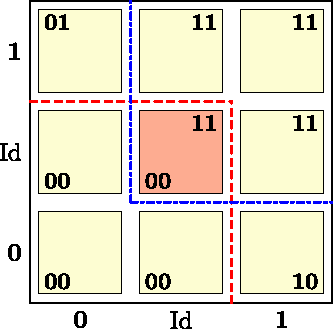
\includegraphics[width=\linewidth]{figures/PG1.pdf}
        \caption{Steady states supported by $MBF(1) \times MBF(1)$}
    \end{figure}
    \end{column}
\end{columns}
\end{adjustwidth}
\footnotetext[1]{
    Models supporting steady states: 
    \begin{tikzpicture}[baseline=-0.75ex]
        \draw[line width=1pt, dashed, red] (0,0) -- (0.5,0);
    \end{tikzpicture} $(00)$, 
    \begin{tikzpicture}[baseline=-0.75ex]
        \draw[line width=1pt, dashdotted, blue] (0,0) -- (0.5,0);
    \end{tikzpicture} $(11)$
}
\end{frame}

\begin{frame}{Steady states - Toggle switch with self-activation}
\begin{adjustwidth}{-5cm}{-5cm}
\begin{columns}
    \begin{column}{0.5\textwidth}
        \only<1-6>{
        \begin{table}
            \centering
            \begin{tabular}{|c|c|c|c|c|}
             \hline 
             Size & (11) & (10) & (01) & (00) \\ \hline
             L & 1 & 3 & 3 & 5 \\
             U & 5 & 3 & 3 & 1 \\
             \hline
            \end{tabular}
        \end{table}
        \vspace{1cm}
        
        Positive Toggle switch with self-activation:
        \begin{itemize}
            \item Total: $f \in MBF(2)\times MBF(2)$ = $36$ models \pause
            \item $(00)$: \pause $f \in L(00)\times L(00)$ = \pause $25$ models
            \pause
            \item $(01)$: $f \in L(01)\times U(01)$ = $9$ model
            \pause
            \item $(10)$: $f \in U(10)\times L(11)$ = $9$ model
            \item $(11)$: $f \in U(11)\times U(11)$ = $25$ models
        \end{itemize}}
        \only<7>{
        Toggle switch with self activation:
        \begin{itemize}
            \item Total: $36$ models
            \item $(10)$: $25$ models
            \item $(00)$: $9$ model
            \item $(11)$: $9$ model
            \item $(01)$: $25$ models
        \end{itemize}
        }
    \end{column}
    \pause[1]
    \begin{column}{0.5\textwidth}
    \begin{figure}
        \centering
        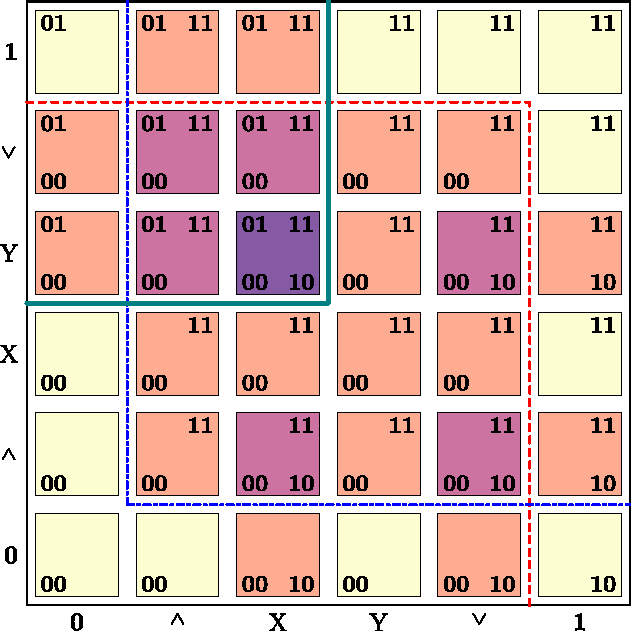
\includegraphics[width=0.9\linewidth]{figures/PG2.pdf}
        \caption{Steady states supported by $MBF(2) \times MBF(2)$}
    \end{figure}
    \end{column}
\end{columns}
\end{adjustwidth}
\footnotetext[1]{
    Models supporting steady states: 
    \begin{tikzpicture}[baseline=-0.75ex]
        \draw[line width=1pt, dashed, red] (0,0) -- (0.5,0);
    \end{tikzpicture} $(00)$, 
    \begin{tikzpicture}[baseline=-0.75ex]
        \draw[line width=1.6pt, teal] (0,0) -- (0.5,0);
    \end{tikzpicture} $(01)$, 
    \begin{tikzpicture}[baseline=-0.75ex]
        \draw[line width=1pt, dashdotted, blue] (0,0) -- (0.5,0);
    \end{tikzpicture} $(11)$
}
\end{frame}

\begin{frame}{Steady states - EMT network}
\only<1>{
    \begin{table}[t]
    \centering
    \begin{tabular}{|c|c|c|}
    \hline 
    State & Parameter sets & MBMs \\
    \hline
    % \beta,200,S,O,Z,34
    % (200,O), (S,Z), (\beta,34), (Z), (200,S,O), (S,Z)\
    Total & $MBF(2) \times MBF(2) \times MBF(2) \times MBF(1) \times MBF(3) \times MBF(2)$ & 77760 \\ \hline 
    (000000) & $L(00) \times L(00) \times L(00) \times L(0) \times L(000) \times L(00)$ & 23750 \\
    (111111) & $U(11) \times U(11) \times U(11) \times U(1) \times U(111) \times U(11)$ & 23750 \\
    (000100) & $L(01) \times L(00) \times L(00) \times U(0) \times L(001) \times L(00)$ & 5250 \\
    (111011) & $U(10) \times U(11) \times U(11) \times L(1) \times U(110) \times U(11)$ & 5250 \\
    (001001) & $L(00) \times L(10) \times U(01) \times L(0) \times L(010) \times U(10)$ & 3780 \\
    (110110) & $U(11) \times U(01) \times L(10) \times U(1) \times U(101) \times L(01)$ & 3780 \\
    (100100) & $U(01) \times L(00) \times L(10) \times U(0) \times L(001) \times L(00)$ & 3150 \\
    (011011) & $L(10) \times U(11) \times U(01) \times L(1) \times U(110) \times U(11)$ & 3150 \\
    \hline
    \end{tabular}
    \caption{Number of MBMs supporting the top 8 most common steady states.}
\end{table}
}
\only<2>{
    \begin{table}[t]
    \centering
    \begin{tabular}{|c|c|c|c|}
    \hline 
    State & MBMs & EMT-state & \\
    \hline
    % \beta,200,S,O,Z,34
    % (200,O), (S,Z), (\beta,34), (Z), (200,S,O), (S,Z)\
    Total & 77760 & & \\ \hline 
    \pause
    (000000) &  23750 & miR200$^+$ OVOL2$^+$ miR34a$^+$ & E \\
    (111111) & 23750 & TGF$\beta^+$ SNAI1$^+$ ZEB1$^+$ & M \\
    (000100) & 5250 & miR200$^+$ miR34a$^+$ & I \\
    (111011) & 5250 & TGF$\beta^+$ SNAI1$^+$ OVOL2$^+$ ZEB1$^+$ & I \\
    (001001) & 3780 & miR200$^+$ SNAI1$^+$ OVOL2$^+$ & I \\
    (110110) & 3780 & TGF$\beta^+$ ZEB1$^+$ miR34a$^+$ & I \\
    (100100) & 3150 & TGF$\beta^+$ miR200$^+$ miR34a$^+$ & I \\
    (011011) & 3150 & SNAI1$^+$ OVOL2$^+$ ZEB1$^+$ & I\\
    \hline
    \end{tabular}
    \caption{Number of MBMs supporting the top 8 most common steady states.}
\end{table}
}
\footnotetext[1]{E: Epithelial, M: Mesenchymal, I: Intermediate}
\end{frame}

\begin{frame}{Bistability}
        Steady states: $d,e \in \bbB^N$ 
        \pause
        \[ f_i \in Z_i(d)\cap Z'_i(e) \]
        \[ Z_i(d)= \left\{ \begin{array}{cc}
        U(d_{\Sources(i)}) & \mbox{ if } \quad d_i=1\\
        L(d_{\Sources(i)}) &\mbox{ if } \quad d_i=0
        \end{array}
        \right .
        \]
        \pause
        \[d_i =e_i \implies Z_i(d) \cap Z'_i(e) \not = \emptyset.\]
        \[d_i\not =e_i \implies Z_i(d) \cap Z'_i(e) \quad \text{may be empty}\]
        Note: Bistability between $d,e$: $d$ and $e$ among the steady states; others may also exist.
        \pause
        
        Most common $\boolf$ and $\boolt$
        \[ \prod_{i=1}^N |MBF(k_i)|-2 \]
    \footnotetext[1]{$d_{\Sources(i)}$ = values of the input nodes of $v_i$ evaluated at the state $d$}
\end{frame}

\begin{frame}{Multistability}
    Steady states: $d^1,\ldots, d^q \in \bbB^N$ 
    \[ f_i \in \bigcap_{j=1}^q Z_i(d^j)\]
    \[ Z_i(d^j)= \left\{ \begin{array}{cc}
    U(d^j_{\Sources(i)}) & \mbox{ if } \quad  d^j_i=1\\
    L(d^j_{\Sources(i)}) &\mbox{ if } \quad  d^j_i=0
    \end{array}
    \right . ,
    \]
    \pause
    \textit{Exact $q$-multistablity}: supports exactly $q$-steady states
    \[ em_q(A) = m_q(A) \setminus \bigcup_{n>q, A \subset E} m_n(E)\]
    \footnotetext[1]{$d^j_{\Sources(i)}$ = values of the input nodes of $v_i$ evaluated at the state $d^j$}
    \footnotetext[2]{$m_n(E)$= MBMs supporting $n-$multistability for $E:=\{e_1, \ldots, e_n\}$}
    \footnotetext[3]{$em_q(A)$= MBMs supporting exact $q-$multistability for $A=\{e_1, \ldots, e_q\}$}
\end{frame}

\begin{frame}{Bistability - Toggle switch}
\begin{adjustwidth}{-5cm}{-5cm}
\begin{columns}
    \begin{column}{0.6\textwidth}
    \only<1-2>{
    Positive Toggle switch:
    \[ d=(00) \quad \text{and} \quad e=(11)\]
    \[ f_1\in L(0) \cap U(1) \quad \mbox{ and } \quad f_1\in L(0) \cap U(1)\]
    \[(Id, Id)\]
    \pause 
    \[ d=(00) \quad \text{and} \quad e=(10)\]
    \[ f_1\in L(0) \cap U(0) \quad \mbox{ and } \quad f_2\in L(0) \cap L(1)\]
    \[L(0) \cap U(0) =\emptyset \rightarrow \text{no MBMs}\]
    }
    \only<3>{
    Toggle switch:
    \begin{itemize}
        \item $(10)$ and $(01)$: 1 model
    \end{itemize}
    }
    \end{column}
    \pause[1]
    \begin{column}{0.3\textwidth}
    \begin{figure}
        \centering
        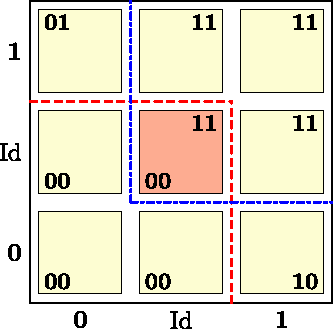
\includegraphics[width=\linewidth]{figures/PG1.pdf}
        \caption{Steady states supported by $MBF(1) \times MBF(1)$}
    \end{figure}
    \end{column}
\end{columns}
\end{adjustwidth}
\footnotetext[1]{ 
    \begin{tikzpicture}[baseline=-0.75ex]
        \definecolor{cellcolor}{RGB}{253,253,210}
        \node[draw,fill=cellcolor] {};
    \end{tikzpicture} Monostable, 
    \begin{tikzpicture}[baseline=-0.75ex]
        \definecolor{cellcolor}{RGB}{253,172,145}
        \node[draw,fill=cellcolor] {};
    \end{tikzpicture} Bistable
}
\end{frame}

\begin{frame}{Bistability - EMT network}
Bistability between E and M states

\[4\times4\times4\times1\times18\times4 = 4608 \text{ MBMs}\] 

Prevalence = $4608/77760=0.059 \approx 6\%$
\end{frame}

\begin{frame}{Bistability \& Multistability - Toggle switch with self-activation}
\begin{adjustwidth}{-5cm}{-5cm}
\begin{columns}
    \begin{column}{0.5\textwidth}
    \only<1-2>{
    Positive Toggle switch with self-activation:
    \[ d=(00) \quad \text{and} \quad e=(11)\]
    \[(L(00) \cap U(11)) \times (L(00) \cap U(11)) = 16 \mbox{ models}\]
    \pause 
    \begin{itemize}
        \item $(00)$ and $(01)$: 6 models
        \item $(00)$ and $(10)$: 6 models
        \item $(01)$ and $(11)$: 6 models
        \item $(10)$ and $(11)$: 6 models
        \item $(01)$ and $(10)$: 1 model
    \end{itemize}
    }
    \only<3>{
    Toggle switch with self-activation:
    \begin{itemize}
        \item $(10)$ and $(01)$: 16 models
        \item $(10)$ and $(11)$: 6 models
        \item $(10)$ and $(00)$: 6 models
        \item $(11)$ and $(01)$: 6 models
        \item $(00)$ and $(01)$: 6 models
        \item $(11)$ and $(00)$: 1 model
    \end{itemize}
    }
    \only<4>{
    Positive Toggle switch with self-activation:
    \begin{itemize}
        \item Tristability:
        \begin{itemize}
            \item $(00, 01, 11)$: 4 models
            \item $(00, 10, 11)$: 4 models
        \end{itemize}
        \item Quadrastability: 
        \begin{itemize}
                \item $(00, 10, 01, 11)$: 1 model
        \end{itemize}
    \end{itemize}
    }
    \only<5>{
    Toggle switch with self-activation:
    \begin{itemize}
        \item Tristability:
        \begin{itemize}
            \item $(10, 11, 01)$: 4 models
            \item $(10, 00, 01)$: 4 models
        \end{itemize}
        \item Quadrastability: 
        \begin{itemize}
            \item $(10, 00, 11, 01)$: 1 model
        \end{itemize}
    \end{itemize}
    }
    \end{column}
    \pause[1]
    \begin{column}{0.5\textwidth}
    \begin{figure}
        \centering
        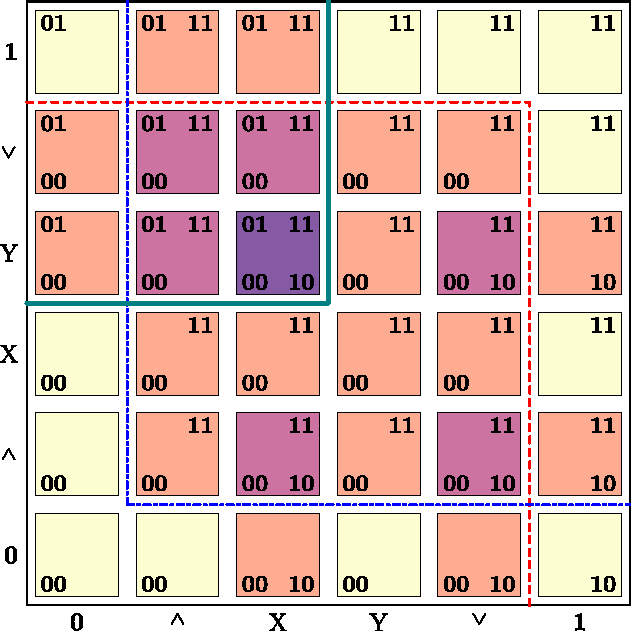
\includegraphics[width=0.9\linewidth]{figures/PG2.pdf}
        \caption{Steady states supported by $MBF(2) \times MBF(2)$}
    \end{figure}
    \end{column}
\end{columns}
\end{adjustwidth}
\footnotetext[1]{Exact multistability: 
    \begin{tikzpicture}[baseline=-0.75ex]
        \definecolor{cellcolor}{RGB}{253,253,210}
        \node[draw,fill=cellcolor] {};
    \end{tikzpicture} Monostable, 
    \begin{tikzpicture}[baseline=-0.75ex]
        \definecolor{cellcolor}{RGB}{253,172,145}
        \node[draw,fill=cellcolor] {};
    \end{tikzpicture} Bistable, 
    \begin{tikzpicture}[baseline=-0.75ex]
        \definecolor{cellcolor}{RGB}{204,115,161}
        \node[draw,fill=cellcolor] {};
    \end{tikzpicture} Tristable, 
    \begin{tikzpicture}[baseline=-0.75ex]
        \definecolor{cellcolor}{RGB}{133,89,163}
        \node[draw,fill=cellcolor] {};
    \end{tikzpicture} Quadrastable
}
\end{frame}

\begin{frame}{Summary}
    \begin{itemize}
        \item Mathematical framework: explore GRN dynamics without simulations
        \pause
        \item Team networks (NL-free) most common states: \\
        A high, B low\\
        A low, B high\\
        Regardless of network size, density as long as coherent
        \pause
        \item Bistability highest between these states
    \end{itemize}
\end{frame}

\begin{frame}{Future Directions}
    \begin{itemize}
        \item Negative loop influence - Complex attractors
        \item Designing networks with certain properties
    \end{itemize}
\end{frame}
\appendix

\begin{frame}{Acknowledgements}
    \begin{adjustwidth}{-5cm}{-5cm}
    \begin{figure}
        \centering
        \begin{subfigure}{0.55\textwidth}
            \centering
            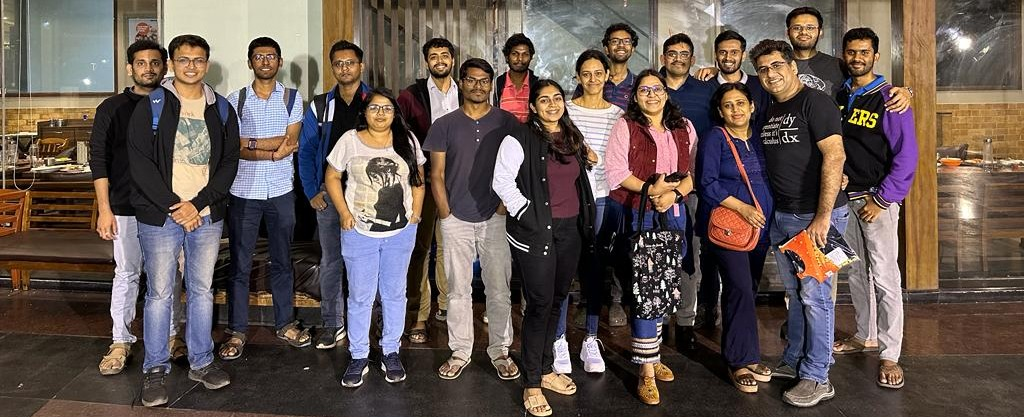
\includegraphics[width=\textwidth]{CSB_Lab}
        \end{subfigure}        
        \begin{subfigure}{0.55\textwidth}
            \centering
            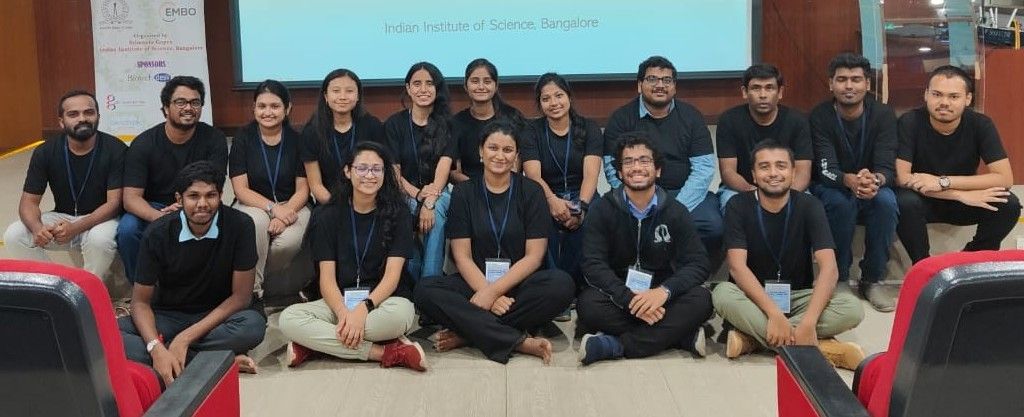
\includegraphics[width=\textwidth]{SG_Lab}
        \end{subfigure}
        \par\bigskip
        \begin{subfigure}{0.25\textwidth}
            \centering
            
\includegraphics[width=\textwidth]{PMRF_Logo}
        \end{subfigure}
    \end{figure}
    \end{adjustwidth}        
\end{frame}

\begin{frame}[standout]
    \Huge{Thank You}
\end{frame}

\begin{frame}[standout]
        
    \begin{figure}
        \centering
        
\includegraphics[width=0.2\linewidth]{DOIQR}
    \end{figure}
    \small{DOI: 10.1101/2025.10.16.682751}
\end{frame}

\end{document}
